\documentclass[8pt,aspectratio=169,xcolor=dvipsnames]{beamer}
\usetheme{SimpleDarkBlue}
\usepackage{hyperref}
\usepackage{graphicx} % Allows including images
\usepackage{amsmath}
\usepackage{bbm}
\usepackage{booktabs} % Allows the use of \toprule, \midrule and \bottomrule in tables
\usepackage{tikz} % For advanced graphics manipulation
\usetikzlibrary{shapes.geometric, arrows, positioning, fit, calc, patterns}
\usepackage{graphicx}
\graphicspath{{figures/}}
% Define colors
\definecolor{backbone}{RGB}{52, 152, 219}      % Blue for backbone
\definecolor{rpn}{RGB}{231, 76, 60}            % Red for RPN
\definecolor{roiheads}{RGB}{155, 89, 182}      % Purple for ROI heads
\definecolor{outputs}{RGB}{46, 204, 113}       % Green for outputs
\definecolor{features}{RGB}{52, 73, 94}        % Dark gray for features
\definecolor{conv}{RGB}{26, 188, 156}          % Teal for conv layers

\definecolor{backbone}{RGB}{200,230,255}
\definecolor{features}{RGB}{255,230,200}
\definecolor{rpn}{RGB}{230,255,200}
\definecolor{roiheads}{RGB}{255,200,230}
\definecolor{conv}{RGB}{220,220,255}
\definecolor{outputs}{RGB}{255,255,200}
\definecolor{grayscale}{RGB}{255,180,180}
\definecolor{slate}{RGB}{112,128,144}
\definecolor{indigo}{RGB}{75,0,130}

% Logo configuration - only for the title page
\titlegraphic{
  \begin{tikzpicture}[remember picture, overlay]
    \node[anchor=north west, inner sep=1.5em] at (current page.north west) {
      \includegraphics[height=1.2cm]{logo2.png}
    };
  \end{tikzpicture}
  \begin{tikzpicture}[remember picture, overlay]
    \node[anchor=north east, inner sep=1.2em] at (current page.north east) {
      \includegraphics[height=1cm]{logo.png}
    };
  \end{tikzpicture}
}

%----------------------------------------------------------------------------------------
%    TITLE PAGE
%---------------------------------------------------------
\title{Advanced Deep Learning for Multi-View \\Structural Reasoning in Mammographic Analysis}
\subtitle{Internship Overview}
\author{Student : Imade Bouftini
\\Supervision : Youssef ALJ}

\date{\today} % Date, can be changed to a custom date
\definecolor{ign}{RGB}{197, 23, 46}
%----------------------------------------------------------------------------------------
%    PRESENTATION SLIDES
%----------------------------------------------------------------------------------------

\begin{document}
\usebackgroundtemplate{\includegraphics[width=\paperwidth,height=\paperheight]{bg.png}}
\begin{frame}
    % Print the title page as the first slide
    \titlepage
\end{frame}
\usebackgroundtemplate{}

\begin{frame}{Overview}
    % Throughout your presentation, if you choose to use \section{} and \subsection{} commands, these will automatically be printed on this slide as an overview of your presentation
    \tableofcontents
\end{frame}

{
\setbeamertemplate{background}{
    \includegraphics[width=\paperwidth,height=\paperheight]{figures/bg2.png}
}
\begin{frame}[plain]

    \vfill
    \begin{center}
    {\color{white}\large Section I}

    \vspace{1cm}

    {\color{white}\bfseries\fontsize{28}{34}\selectfont Introduction}
    \end{center}
    \vfill

\end{frame}

\setbeamertemplate{background}{} % Reset background
}

\section{Clinical Context \& Problem Statement}

\begin{frame}{Clinical Context: Breast Cancer Screening}
    \framesubtitle{Global Impact and Detection Methodology}
    
    \begin{itemize}
        \item Breast cancer affects millions worldwide (2.3M new cases annually)
        \item Early detection can reduce mortality by 20-40\%
        \item Mammography is the primary screening tool
    \end{itemize}
    \begin{center}
    \begin{tabular}{ccc}
    \includegraphics[width=0.55\textwidth]{mammograph.png} &\quad& \includegraphics[width=0.32\textwidth]{mammogram.png} \\
    Imaging protocol \href{https://theses.hal.science/tel-03677490v1/file/M_TARDY.pdf}{[Source]} &\quad& Mammogram Views (MLO/CC) \\
    \end{tabular}
    \end{center}
\end{frame}



\begin{frame}{Clinical Context: Detection Challenges}
    \framesubtitle{Balancing Sensitivity and Specificity in Screening}
    
\begin{figure}
    \centering
    \includegraphics[width=0.5\linewidth]{dense.png}
    \caption{Mammograms with various density levels \href{https://www.mdpi.com/2313-433X/9/5/95}{[Source]}}
    \label{fig:enter-label}
\end{figure}
    \begin{center}
        \textbf{Clinical Challenges:}
        \begin{itemize}
            \item Diverse tissue density and appearance variation between patients
            \item Extremely low prevalence ($\sim 0.5\%$  in screening populations)
            \item Subtle presentation of early-stage cancers
        \end{itemize}
        
        \vspace{0.3cm}
        \begin{columns}[c]
            \column{0.45\textwidth}
            \textcolor{red}{False negatives} cause:
                \begin{itemize}
                    \item Delayed diagnosis 
                    \item Poorer prognosis
                    \item Increased treatment costs
                \end{itemize}
            
            \column{0.45\textwidth}
            \textcolor{OliveGreen}{False positives} cause:
                \begin{itemize}
                    \item Unnecessary biopsies
                    \item Patient anxiety and stress
                    \item Healthcare resource burden
                \end{itemize}
        \end{columns}
    \end{center}
 \end{frame}

\begin{frame}{Clinical Context: Multi-View Integration}
    \framesubtitle{Mimicking Radiologist Reasoning with Multiple Views}
    
    \begin{alertblock}{Core Challenge}
How can we leverage ipsilateral and bilateral views to replicate the natural reasoning ability of radiologists in breast cancer detection?
    \end{alertblock}
\begin{figure}
    \centering
    \includegraphics[width=0.8\linewidth]{views.png}
    \caption{Illustration of the relation among mammography views \href{https://arxiv.org/abs/2105.10160}{[Source]}}
    \label{fig:enter-label}
\end{figure}
\end{frame}





%----------------------------------------------------------------------------------------
{
\setbeamertemplate{background}{
    \includegraphics[width=\paperwidth,height=\paperheight]{figures/bg2.png}
}
\begin{frame}[plain]

    \vfill
    \begin{center}
    {\color{white}\large Section II}

    \vspace{1cm}

    {\color{white}\bfseries\fontsize{28}{34}\selectfont Single-view detection}
    \end{center}
    \vfill

\end{frame}
\setbeamertemplate{background}{} % Reset background
}

\section{Single-view detection}

\begin{frame}{SOTA Single-View Detection Models}
\begin{center}
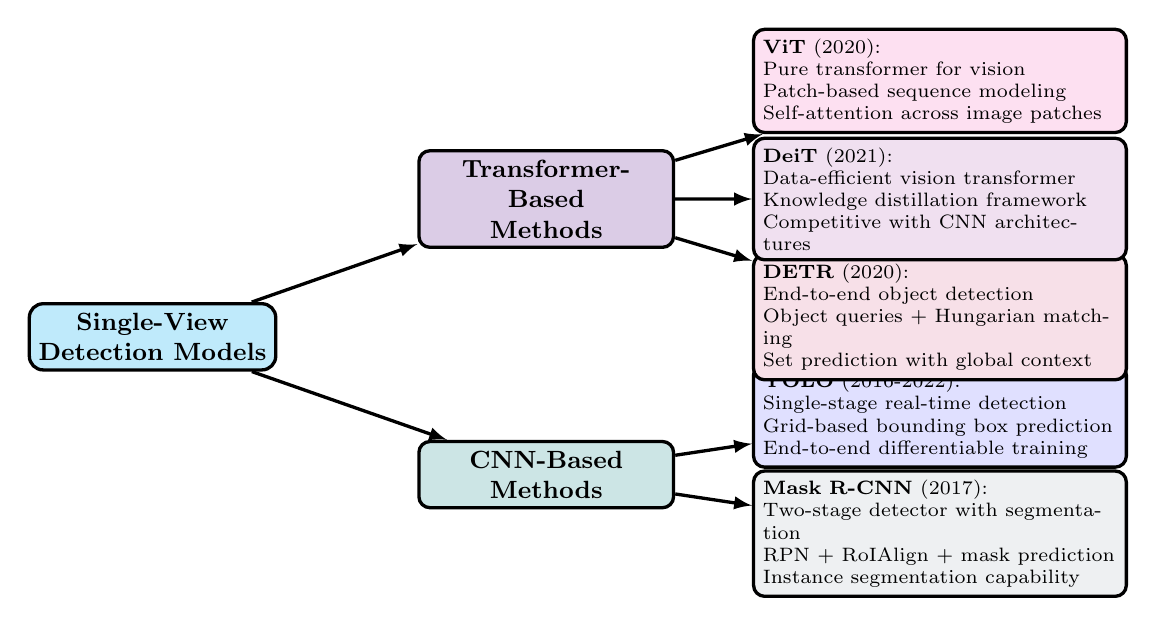
\begin{tikzpicture}[
    grow=right,
    level distance=5cm,
    level 1/.style={sibling distance=3.5cm},
    level 2/.style={sibling distance=1.5cm},
    level 1/.append style={
        every node/.style={minimum width=2cm, text width=3cm, font=\scriptsize, align=center, rounded corners=4pt, draw, line width=1.2pt}
    },
    level 2/.append style={
        every node/.style={rounded corners=4pt, draw, align=left, line width=1.2pt,
                           minimum height=0.9cm, font=\scriptsize, text width=4.5cm}
    },
    edge from parent/.style={draw, -latex, thick, line width=1.2pt}
]
    % Root node with modern gradient-like effect
    \node[minimum width=2.8cm, fill=cyan!25, align=center, draw, line width=1.2pt, 
          text=black, font=\small\bfseries, rounded corners=5pt] {Single-View\\Detection Models}
        % Level 1: Categories with cool color scheme
        child {node[minimum width=2.8cm, fill=teal!20, align=center, text=black, font=\small\bfseries] {CNN-Based\\Methods}
            child {node[fill=slate!12, text=black] {\textbf{Mask R-CNN} (2017):\\
            Two-stage detector with segmentation\\
            RPN + RoIAlign + mask prediction\\
            Instance segmentation capability}}
            child {node[fill=blue!12, text=black] {\textbf{YOLO} (2016-2022):\\
            Single-stage real-time detection\\
            Grid-based bounding box prediction\\
            End-to-end differentiable training}}
        }
        child {node[minimum width=2.8cm, fill=indigo!20, align=center, text=black, font=\small\bfseries] {Transformer-Based\\Methods}
            child {node[fill=purple!12, text=black] {\textbf{DETR} (2020):\\
            End-to-end object detection\\
            Object queries + Hungarian matching\\
            Set prediction with global context}}
            child {node[fill=violet!12, text=black] {\textbf{DeiT} (2021):\\
            Data-efficient vision transformer\\
            Knowledge distillation framework\\
            Competitive with CNN architectures}}
            child {node[fill=magenta!12, text=black] {\textbf{ViT} (2020):\\
            Pure transformer for vision\\
            Patch-based sequence modeling\\
            Self-attention across image patches}}
        };
\end{tikzpicture}
\end{center}
\end{frame}

\begin{frame}<1-8>{Mask R-CNN}

\tikzset{
  onslide/.code args={<##1>##2}{%
    \only<##1>{\pgfkeysalso{##2}}%
  }
}

% Architecture diagram
\centering
\begin{tikzpicture}[
    scale=0.65, transform shape,
    node distance=1.5cm,
    block/.style={rectangle, draw, thick, minimum height=1cm, minimum width=1.4cm, text centered, font=\scriptsize, rounded corners=2pt, align=center},
    smallblock/.style={rectangle, draw, thick, minimum height=0.7cm, minimum width=1cm, text centered, font=\tiny, rounded corners=2pt, align=center},
    convblock/.style={rectangle, draw, thick, minimum height=0.6cm, minimum width=0.6cm, text centered, font=\tiny, rounded corners=2pt, align=center},
    arrow/.style={->,>=stealth,thick}
]

% Define colors


% Main pipeline nodes
\node[block, fill=gray!20] (input) at (0,0) {\textbf{Input}\\Mammogram\\(1024×1024×1)};
\node[block, fill=backbone,onslide=<1>{opacity=1}, onslide=<-1>{opacity=0.2}] (backbone) at (3.2,0) {\textbf{ResNet-50}\\+ FPN};
\node[block, fill=features,onslide=<3>{opacity=1}, onslide=<-3>{opacity=0.2}] (features) at (6.0,0) {\textbf{Feature Maps}\\$P_2$ to $P_6$};
\node[block, fill=rpn,onslide=<3>{opacity=1}, onslide=<-3>{opacity=0.2}] (rpn) at (6.0,1.5) {\textbf{RPN}\\Region\\Proposals};
\node[block, fill=roiheads!30,onslide=<4>{opacity=1}, onslide=<-4>{opacity=0.2}] (roialign) at (8.8,0) {\textbf{RoIAlign}\\$(7 \times 7)$};
\node[block, fill=roiheads,onslide=<5>{opacity=1}, onslide=<-5>{opacity=0.2}] (roi_fc) at (11.6,0) {\textbf{FC Layers}};
\node[block, fill=gray!20,onslide=<7>{opacity=1}, onslide=<-7>{opacity=0.2}] (output_vis) at (17.2,0) {\textbf{Final Output}\\Detection\\+ Segmentation};



% Output branches
\node[smallblock, fill=outputs,onslide=<5>{opacity=1}, onslide=<-5>{opacity=0.2}] (box_output) at (14.4,1.4) {\textbf{Box}\\Regression};
\node[smallblock, fill=outputs,onslide=<5>{opacity=1}, onslide=<-5>{opacity=0.2}] (class_output) at (14.4,0) {\textbf{Class}\\Prediction};

% Mask branch
\node[convblock, fill=conv,onslide=<6>{opacity=1}, onslide=<-6>{opacity=0.2}] (conv1) at (11.6,-1.8) {\textbf{Conv}\\$3\times3$};
\node[convblock, fill=conv,onslide=<6>{opacity=1}, onslide=<-6>{opacity=0.2}] (conv2) at (12.6,-1.8) {\textbf{Conv}\\$3\times3$};
\node[convblock, fill=conv,onslide=<6>{opacity=1}, onslide=<-6>{opacity=0.2}] (conv3) at (13.6,-1.8) {\textbf{Conv}\\$3\times3$};
\node[smallblock, fill=outputs,onslide=<6>{opacity=1}, onslide=<-6>{opacity=0.2}] (mask_output) at (15.4,-1.8) {\textbf{Mask}\\Prediction};

% Main flow arrows
\draw[arrow,onslide=<1>{opacity=1}, onslide=<-1>{opacity=0.2}] (input.east) -- (backbone.west);
\draw[arrow,onslide=<3>{opacity=1}, onslide=<-3>{opacity=0.2}] (backbone.east) -- (features.west);
\draw[arrow,onslide=<4>{opacity=1}, onslide=<-4>{opacity=0.2}] (features.east) -- (roialign.west);
\draw[arrow,onslide=<5>{opacity=1}, onslide=<-5>{opacity=0.2}] (roialign.east) -- (roi_fc.west);

% RPN branch arrows
\draw[arrow,onslide=<3>{opacity=1}, onslide=<-3>{opacity=0.2}] (features.north) -| (rpn.south);
\draw[arrow,onslide=<4>{opacity=1}, onslide=<-4>{opacity=0.2}] (rpn.east) -| (roialign.north);

% Output branch arrows
\draw[arrow,onslide=<5>{opacity=1}, onslide=<-5>{opacity=0.2}] (roi_fc.north) |- (box_output.west);
\draw[arrow,onslide=<5>{opacity=1}, onslide=<-5>{opacity=0.2}] (roi_fc.east) -- (class_output.west);

% Mask branch arrows
\draw[arrow,onslide=<6>{opacity=1}, onslide=<-6>{opacity=0.2}] (roialign.south) |- (conv1.west);
\draw[arrow,onslide=<6>{opacity=1}, onslide=<-6>{opacity=0.2}] (conv1.east) -- (conv2.west);
\draw[arrow,onslide=<6>{opacity=1}, onslide=<-6>{opacity=0.2}] (conv2.east) -- (conv3.west);
\draw[arrow,onslide=<6>{opacity=1}, onslide=<-6>{opacity=0.2}] (conv3.east) -- (mask_output.west);

% Final output arrows
\draw[arrow,onslide=<7>{opacity=1}, onslide=<-7>{opacity=0.2}] (box_output.east) -| (output_vis.north);
\draw[arrow,onslide=<7>{opacity=1}, onslide=<-7>{opacity=0.2}] (class_output.east) -- (output_vis.west);
\draw[arrow,onslide=<7>{opacity=1}, onslide=<-7>{opacity=0.2}] (mask_output.east) -| (output_vis.south);

\end{tikzpicture}

\only<1>{
\centering
\vspace{0.5em}
\textbf{Step 1: Data Preparation}

\begin{columns}[T]
\begin{column}{0.48\textwidth}
\begin{block}{Data Loading}
\small
\textbf{Mammogram Standardization:}
\begin{itemize}
\item Let $I_{\text{raw}} \in \mathbb{N}^{H\times W}$ coded in \texttt{uint16}
\item Normalized image: $I_{\text{norm}} = \frac{I_{\text{raw}}}{65535}$ then $I_{\text{norm2}} = \frac{I_{\text{norm} }-m_{imagenet}}{\sigma_{imagenet}}$ 

\item Resized to $1024 \times 1024$
\end{itemize}
\end{block}
\end{column}

\begin{column}{0.48\textwidth}
\begin{block}{Medical Augmentation Pipeline}
\small
    \begin{itemize}
        \item \textbf{Elastic Distortion}: tissue deformation and compression variations
        \item \textbf{RandomGamma}: exposure variations between mammographs
        \item \textbf{GaussianBlur}: focus variations
        \item \textbf{GaussNoise}: sensor noise
        \item \textbf{RandomBrightnessContrast}: illumination differences
        \item \textbf{Geometric transformations}: handle different orientations
    \end{itemize}
\end{block}
\end{column}
\end{columns}
}

\only<2>{
\centering
\vspace{0.5em}
\textbf{Step 2: Backbone Feature Extraction (ResNet-50)}
\begin{columns}[T]
\begin{column}{0.48\textwidth}
\begin{block}{ResNet-50}
\small
\textbf{Backbone:} Extracts high-level semantic features using a ResNet-50 pretrained on ImageNet.\\[0.5em]

\textbf{Residual Blocks:} Solve the vanishing gradient problem by adding skip connections.

\begin{center}
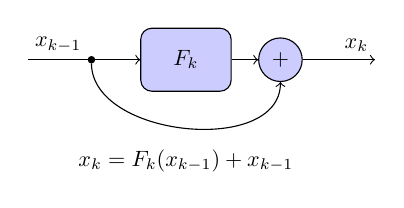
\begin{tikzpicture}[node distance=1.5cm, auto, scale=0.8, every node/.style={transform shape}]
    % Styles
    \tikzstyle{block} = [rectangle, draw, fill=blue!20, 
                        text width=1.2cm, text centered, rounded corners, minimum height=1cm]
    \tikzstyle{sum} = [draw, fill=blue!20, circle, minimum size=0.6cm]
    \tikzstyle{junction} = [draw, fill=black, circle, minimum size=0.1cm, inner sep=0pt]

    % Nodes
    \node at (0,0) [junction] (j) {};
    \node [block, right of=j] (Fk) {$F_k$};
    \node [sum, right of=Fk] (sumk) {$+$};
    \coordinate [right of=sumk, node distance=1.5cm] (out) {};
    
    % Connections
    \draw[-] ($(j) - (1.0cm,0)$) -- node[above] {$x_{k-1}$} (j);
    \draw[->] (j) -- (Fk);
    \draw[->] (Fk) -- (sumk);
    \draw[->] (sumk) -- node[above, xshift=8pt] {$x_k$} (out);
    \draw[->] (j) to[out=-90, in=-90] (sumk);

    % Formula node inside TikZ
    \node[below=0.8cm of Fk] {$x_k = F_k(x_{k-1}) + x_{k-1}$};
\end{tikzpicture}
\end{center}
\end{block}
\end{column}


\begin{column}{0.48\textwidth}
\begin{block}{Transform Parameters}
\small

\textbf{Input Adaptation for Grayscale:}
\begin{itemize}
  \item ImageNet weights assume RGB input.
  \item Grayscale adaptation via channel-wise averaging:
  $$W_{\text{gray}} = 0.299 .W_R + 0.587.W_G + 0.114.W_B$$
\end{itemize}
\end{block}
\end{column}
\end{columns}
}

\only<3>{
\centering
\vspace{0.5em}
\textbf{Step 3: Feature Pyramid Network (FPN)}

\begin{columns}[T]
\begin{column}{0.48\textwidth}
\begin{block}{Feature Pyramid Network}
\small

\textbf{Bottom-up:} $C_2$ to $C_5$ with strides $\{4,8,16,32\}$

\textbf{Top-Down Path:} $P_i = C_i + \text{Upsample}(P_{i+1})$

\textbf{Multi-Scale Features:}
\begin{itemize}
\item $P_2$: Microcalcifications (5-15px)
\item $P_3$: Small masses (15-40px)
\item $P_4$: Medium masses (40-100px)
\item $P_5$: Large masses (100-250px)
\end{itemize}
\end{block}
\end{column}

\begin{column}{0.48\textwidth}
\begin{figure}
    \centering
    \includegraphics[width=\linewidth]{fpn_overview.png}
    \caption{FPN architecture overview}
    \label{fig:enter-label}
\end{figure}
\end{column}
\end{columns}
}

\only<4>{
\centering
\vspace{0.5em}
\textbf{Step 4: Region Proposal Network (RPN)}

\begin{columns}[T]
\begin{column}{0.48\textwidth}

\begin{figure}
    \centering
    \includegraphics[width=\linewidth]{rpn.png}
    \caption{RPN architecture overview}
    \label{fig:enter-label}
\end{figure}
\end{column}

\begin{column}{0.48\textwidth}
\begin{block}{RPN Loss Function}
\small
$$L_{rpn} = \frac{1}{N_{cls}}\sum_i L_{cls}(p_i, p_i^*) + \frac{\lambda}{N_{reg}}\sum_i p_i^* L_{reg}(t_i, t_i^*)$$

\begin{itemize}
\item $L_{reg}(t, t^*) = \mathrm{smooth}_{\ell_{1}}(t - t^*)$
\item $L_{cls}(p_i, p_i^*) = -p_i* log(p_i) - (1-p_i^*) log(1-p_i)$
\end{itemize}
\end{block}
\end{column}
\end{columns}
}

\only<5>{
\centering
\vspace{0.5em}
\textbf{Step 5: RoIAlign}

\begin{columns}[T]
\begin{column}{0.48\textwidth}
\begin{block}{RoIAlign Implementation}
\small
\textbf{Bilinear Interpolation:}
$$f(x,y) = \sum_{i,j} f(i,j) \max(0, 1-|x-i|) \max(0, 1-|y-j|)$$
\textbf{Quantization-Free Alignment:}
\begin{itemize}
\item No coordinate snapping
\item Sub-pixel accuracy maintained
\item $7\times7$ output resolution
\item Critical for mask precision
\end{itemize}
\end{block}
\end{column}

\begin{column}{0.48\textwidth}
\begin{figure}
    \centering
    \includegraphics[width=0.8\linewidth]{roialign.png}
    \caption{RoIAlign illustration example}
    \label{fig:enter-label}
\end{figure}
\end{column}
\end{columns}
}


\only<6>{
\centering
\vspace{0.5em}
\textbf{Step 6: Classification and Box Regression}

\begin{columns}[T]
\begin{column}{0.48\textwidth}
\begin{block}{Classification + Box Regression}
\small
\textbf{FC Architecture:}
$$p = \text{softmax}(W_{cls} \cdot f + b_{cls})$$
$$\Delta = W_{box} \cdot f + b_{box}$$
\textbf{Network Structure:}
\begin{itemize}
\item FC1: $7\times7\times256 \rightarrow 1024$
\item FC2: $1024 \rightarrow 1024$
\item Class output: $1024 \rightarrow 2$ (background + mass)
\item Box output: $1024 \rightarrow 4$ coordinates
\end{itemize}
\end{block}
\end{column}

\begin{column}{0.48\textwidth}
\begin{block}{Box Parameterization}
\small
\textbf{Regression Targets:}
\begin{itemize}
\item $t_x = (x - x_a)/w_a$
\item $t_y = (y - y_a)/h_a$
\item $t_w = \log(w/w_a)$
\item $t_h = \log(h/h_a)$
\end{itemize}
\textbf{Smooth $\ell_1$ and CE as losses}

\end{block}
\end{column}
\end{columns}
}

\only<7>{
\centering
\vspace{0.5em}
\textbf{Step 7: Segmentation}

\begin{columns}[T]
\begin{column}{0.48\textwidth}
\begin{block}{Mask Head Architecture}
\small
\textbf{Convolutional Stack:}
\begin{itemize}
\item 4x Conv3x3-256-ReLU layers
\item Deconv2x2: $256 \rightarrow 2$ classes
\item Output: $14\times14\times2$ binary masks
\item Per-class mask prediction
\item Sigmoid activation for binary output
\end{itemize}
\end{block}
\end{column}

\begin{column}{0.48\textwidth}
\begin{block}{Mask Loss}
\small
$$L_{mask} = -\frac{1}{m^2}\sum_{i,j} [y_{ij}\log(\hat{y}_{ij}) + (1-y_{ij})\log(1-\hat{y}_{ij})]$$
 \begin{itemize}
\item Computed only for positive ROIs
\item Binary cross-entropy per pixel
\end{itemize}
\end{block}
\end{column}
\end{columns}
}

\only<8>{
\centering
\vspace{0.5em}
\textbf{Step 8: Training on Multi-Task Loss}

\begin{columns}[T]
\begin{column}{0.48\textwidth}
\begin{block}{Multi-Task Loss}
\small
$$L_{total} = L_{rpn} + L_{det} +  L_{mask}$$
\textbf{Training Configuration:}
\begin{itemize}
\item Weight decay: $10^{-4}$
\item Momentum: $0.9$
\item Gradient clipping: $\lVert\nabla\rVert\leq 1.0$
\item Batch size: $2$ images
\end{itemize}
\end{block}
\end{column}

\begin{column}{0.48\textwidth}
\begin{block}{3-stage training}
\small
\begin{enumerate}
 \item heads for 10 epochs (LR=0.002)
 \item Initial backbone layers (LR=0.0005) 
 \item Full network for 5 epochs (LR=0.0001)

\end{enumerate}
\end{block}
\end{column}
\end{columns}
}

\end{frame}


%----------------------------------------------------------------------------------------
{
\setbeamertemplate{background}{
    \includegraphics[width=\paperwidth,height=\paperheight]{figures/bg2.png}
}
\begin{frame}[plain]

    \vfill
    \begin{center}
    {\color{white}\large Section III}

    \vspace{1cm}

    {\color{white}\bfseries\fontsize{28}{34}\selectfont Multi-view detection}
    \end{center}
    \vfill

\end{frame}
\setbeamertemplate{background}{} % Reset background
}

\section{Multi-view detection}
\begin{frame}{SOTA Multi-View Detection Models}
\begin{center}
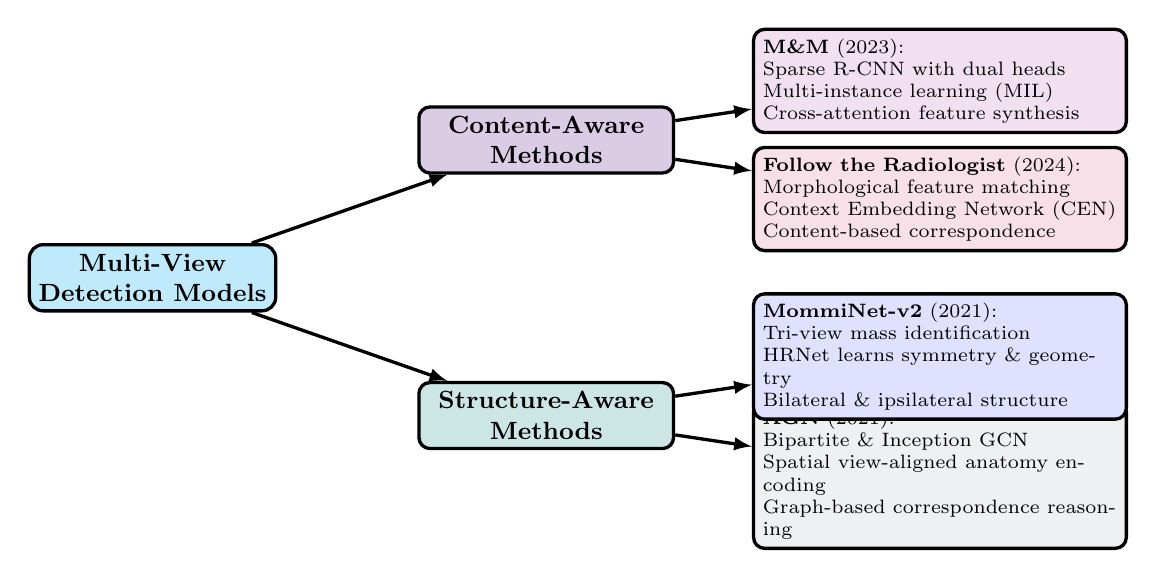
\begin{tikzpicture}[
    grow=right,
    level distance=5cm,
    level 1/.style={sibling distance=3.5cm},
    level 2/.style={sibling distance=1.5cm},
    level 1/.append style={
        every node/.style={minimum width=2cm, text width=3cm, font=\scriptsize, align=center, rounded corners=4pt, draw, line width=1.2pt}
    },
    level 2/.append style={
        every node/.style={rounded corners=4pt, draw, align=left, line width=1.2pt,
                           minimum height=0.9cm, font=\scriptsize, text width=4.5cm}
    },
    edge from parent/.style={draw, -latex, thick, line width=1.2pt}
]
    % Root node with modern gradient-like effect
    \node[minimum width=2.8cm, fill=cyan!25, align=center, draw, line width=1.2pt, 
          text=black, font=\small\bfseries, rounded corners=5pt] {Multi-View\\Detection Models}
        % Level 1: Categories with cool color scheme
        child {node[minimum width=2.8cm, fill=teal!20, align=center, text=black, font=\small\bfseries] {Structure-Aware\\Methods}
            child {node[fill=slate!12, text=black] {\textbf{AGN} (2021):\\
            Bipartite \& Inception GCN\\
            Spatial view-aligned anatomy encoding\\
            Graph-based correspondence reasoning}}
            child {node[fill=blue!12, text=black] {\textbf{MommiNet-v2} (2021):\\
            Tri-view mass identification\\
            HRNet learns symmetry \& geometry\\
            Bilateral \& ipsilateral structure}}
        }
        child {node[minimum width=2.8cm, fill=indigo!20, align=center, text=black, font=\small\bfseries] {Content-Aware\\Methods}
            child {node[fill=purple!12, text=black] {\textbf{Follow the Radiologist} (2024):\\
            Morphological feature matching\\
            Context Embedding Network (CEN)\\
            Content-based correspondence}}
            child {node[fill=violet!12, text=black] {\textbf{M\&M} (2023):\\
            Sparse R-CNN with dual heads\\
            Multi-instance learning (MIL)\\
            Cross-attention feature synthesis}}
        };
\end{tikzpicture}
\end{center}
\end{frame}

\begin{frame}{MaskRCNN adaptation for multi-view detection}
    % Architecture diagram
\centering
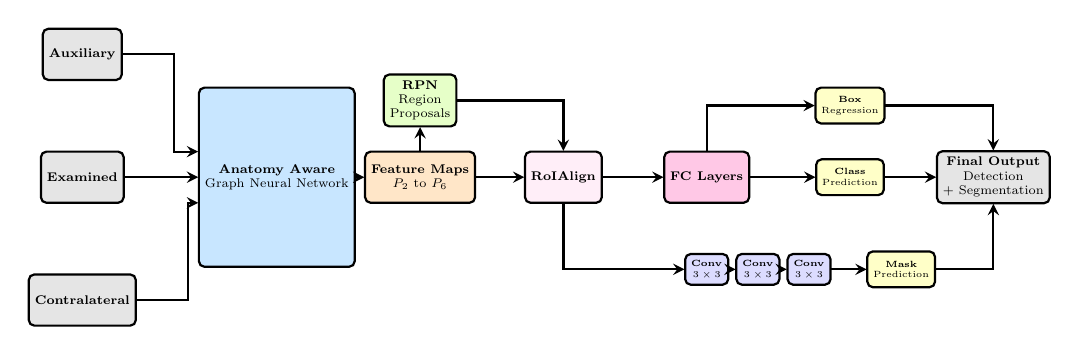
\begin{tikzpicture}[
    scale=0.65, transform shape,
    node distance=1.5cm,
    block/.style={rectangle, draw, thick, minimum height=1cm, minimum width=1.4cm, text centered, font=\scriptsize, rounded corners=2pt, align=center},
    smallblock/.style={rectangle, draw, thick, minimum height=0.7cm, minimum width=1cm, text centered, font=\tiny, rounded corners=2pt, align=center},
    convblock/.style={rectangle, draw, thick, minimum height=0.6cm, minimum width=0.6cm, text centered, font=\tiny, rounded corners=2pt, align=center},
    arrow/.style={->,>=stealth,thick}
]

% Input nodes (three blocks)
\node[block, fill=gray!20] (auxiliary) at (0,2.4) {\textbf{Auxiliary}};
\node[block, fill=gray!20] (examined)  at (0,0)   {\textbf{Examined}};
\node[block, fill=gray!20] (contralateral) at (0,-2.4) {\textbf{Contralateral}};

% Backbone (renamed)
\node[block, fill=backbone, minimum height=3.5cm] (backbone) at (3.8,0) {\textbf{Anatomy Aware}\\Graph Neural Network};

% Remaining nodes unchanged
\node[block, fill=features] (features) at (6.6,0) {\textbf{Feature Maps}\\$P_2$ to $P_6$};
\node[block, fill=rpn] (rpn) at (6.6,1.5) {\textbf{RPN}\\Region\\Proposals};
\node[block, fill=roiheads!30] (roialign) at (9.4,0) {\textbf{RoIAlign}};
\node[block, fill=roiheads] (roi_fc) at (12.2,0) {\textbf{FC Layers}};
\node[block, fill=gray!20] (output_vis) at (17.8,0) {\textbf{Final Output}\\Detection\\+ Segmentation};

% Output branches
\node[smallblock, fill=outputs] (box_output) at (15.0,1.4) {\textbf{Box}\\Regression};
\node[smallblock, fill=outputs] (class_output) at (15.0,0) {\textbf{Class}\\Prediction};

% Mask branch
\node[convblock, fill=conv] (conv1) at (12.2,-1.8) {\textbf{Conv}\\$3\times3$};
\node[convblock, fill=conv] (conv2) at (13.2,-1.8) {\textbf{Conv}\\$3\times3$};
\node[convblock, fill=conv] (conv3) at (14.2,-1.8) {\textbf{Conv}\\$3\times3$};
\node[smallblock, fill=outputs] (mask_output) at (16.0,-1.8) {\textbf{Mask}\\Prediction};

% Arrows from inputs to backbone (orthogonal)
\draw[arrow] (auxiliary.east) -- ++(1,0) |- (backbone.west |- 3.5,0.5);
\draw[arrow] (examined.east) -- ++(1.4,0) |- (backbone.west);
\draw[arrow] (contralateral.east) -- ++(1,0) |- (backbone.west |- -3.5,-0.5);


% Main flow arrows
\draw[arrow] (backbone.east) -- (features.west);
\draw[arrow] (features.east) -- (roialign.west);
\draw[arrow] (roialign.east) -- (roi_fc.west);

% RPN branch arrows
\draw[arrow] (features.north) -| (rpn.south);
\draw[arrow] (rpn.east) -| (roialign.north);

% Output branch arrows
\draw[arrow] (roi_fc.north) |- (box_output.west);
\draw[arrow] (roi_fc.east) -- (class_output.west);

% Mask branch arrows
\draw[arrow] (roialign.south) |- (conv1.west);
\draw[arrow] (conv1.east) -- (conv2.west);
\draw[arrow] (conv2.east) -- (conv3.west);
\draw[arrow] (conv3.east) -- (mask_output.west);

% Final output arrows
\draw[arrow] (box_output.east) -| (output_vis.north);
\draw[arrow] (class_output.east) -- (output_vis.west);
\draw[arrow] (mask_output.east) -| (output_vis.south);

\end{tikzpicture}
\\
\vspace{1cm}
To enable multi-view reasoning, \textcolor{OliveGreen}{\textbf{we replace the standard backbone with an Anatomy-Aware GCN}} that fuses auxiliary/contralateral features into the examined view

\end{frame}

\begin{frame}{Anatomy-aware Graph Network: Core Idea}
\begin{columns}
    \column{0.5\textwidth}
        \begin{figure}
        \centering
        \includegraphics[width=\linewidth]{AGN.png}
        \caption{AGN architecture \href{https://arxiv.org/abs/2105.10160}{[Source]}}
        \label{fig:enter-label}
    \end{figure}

    \column{0.5\textwidth}
    \begin{block}{Key Idea}
    AGN models \textbf{multi-view anatomical reasoning} by explicitly encoding correspondences across:
    \begin{itemize}
        \item \textbf{Ipsilateral views} (CC \& MLO of the same breast)
        \item \textbf{Bilateral views} (CC-left vs. CC-right or MLO-left vs. MLO-right)
    \end{itemize}
    \end{block}

    \begin{block}{Key structure}
    The network uses two Graph Convolutional Networks (GCNs):
    \begin{itemize}
        \item \textcolor{orange}{\textbf{BGN}}: Bipartite Graph for ipsilateral reasoning
        \item \textcolor{ign}{\textbf{IGN}}: Inception Graph for bilateral symmetry analysis
    \end{itemize}
    \end{block}
\end{columns}
\end{frame}

\begin{frame}{Graph construction : Pseudo landmarks}
\begin{columns}
    \column{0.5\textwidth}
    \begin{figure}
        \centering
        \includegraphics[width=0.8\linewidth]{landmarks.png}
        \caption{Pseudo landmarks in MLO/CC views
        \href{https://arxiv.org/abs/2105.10160}{[Source]}}
        \label{fig:enter-label}
    \end{figure}

    \column{0.5\textwidth}
    \begin{block}{Definition}
    Pseudo landmarks $\mathcal{V} = \{v_i\}_{i=1}^N$ are consistent reference points on mammograms.
    \end{block}

    \begin{itemize}
        \item Placed using anatomical priors: nipple, pectoral line and breast contour
        \item Ensure consistent correspondence across patients
        \item Used to define nodes in both GCNs
    \end{itemize}

    \begin{alertblock}{Why Not Grids?}
    Uniform grids are sensitive to scale, shape, and orientation. Pseudo landmarks preserve anatomical semantics.
    \end{alertblock}
\end{columns}
\end{frame}


\begin{frame}{Landmark Detection: Breast Contour Detection}
    \framesubtitle{Otsu Thresholding and B-spline Smoothing}
    
    \begin{columns}
        \begin{column}{0.55\textwidth}
            \footnotesize
            \textbf{1. Breast Region Segmentation (Otsu's Method):}
            \begin{equation}
            t^* = \underset{t}{\arg\max}\{\omega_0(t)\omega_1(t)[\mu_0(t) - \mu_1(t)]^2\}
            \end{equation}
        
            
            \vspace{0.2cm}
            
            \textbf{2. Contour Smoothing (B-spline):}
            \begin{equation}
            S(u) = \sum_{i=0}^{n-1} P_i B_i(u)
            \end{equation}
            
            \textbf{Optimization objective:}
            \begin{equation}
            \min_S \left\{ \sum_{i=1}^n |C_i - S(u_i)|^2 + s \int_0^1 |S''(u)|^2 du \right\}
            \end{equation}
            
            \textbf{Adaptive smoothing parameter:}
            \begin{equation}
            s = \begin{cases}
                10^7 & \text{if view = MLO} \\
                100 & \text{if view = CC}
            \end{cases}
            \end{equation}
        \end{column}
        
        \begin{column}{0.45\textwidth}
            \centering
            \includegraphics[width=0.7\textwidth]{contour.png}
            
            \tiny
            \textit{Contour extraction and smoothing: Raw extracted contour vs. smoothed contour with B-spline interpolation}
        \end{column}
    \end{columns}
    
\end{frame}

\begin{frame}{Landmark Detection: Nipple Detection}
    \framesubtitle{Geometric Principles and Curvature Analysis}
    
    \begin{columns}
        \begin{column}{0.55\textwidth}
            \footnotesize
            \textbf{1. CC View Detection (Lateralmost Point):}
            \begin{equation}
            p_{nipple} = \begin{cases}
               \arg\min_i x_i & \text{if side = Right} \\
                \arg\max_i x_i & \text{if side = Left}
            \end{cases}
            \end{equation}
            
            \vspace{0.2cm}
            
            \textbf{2. MLO View Detection:}
            
            \textbf{Candidate Selection (Lower Lateral Quadrant):}
            \begin{equation}
            \begin{cases}
                x \geq 0.75w \text{ and } y \geq 0.5h & \text{if Left} \\
                x \leq 0.25w \text{ and } y \geq 0.5h & \text{if Right}
            \end{cases}
            \end{equation}
            
            \textbf{Curvature Analysis:}
            \begin{equation}
            \kappa(u) = \frac{x'(u)y''(u) - y'(u)x''(u)}{(x'(u)^2 + y'(u)^2)^{3/2}}
            \end{equation}
            
            \textbf{Optimal Selection:}
            \begin{equation}
            \text{score}(i) = |\kappa(u_i)|
            \end{equation}
        \end{column}
        
        \begin{column}{0.45\textwidth}
            \centering
            \includegraphics[width=\textwidth]{nipple.png}
            
            \tiny
            \textit{Nipple detection: (a) MLO curvature analysis with candidates (green) and final nipple (red) (b) CC lateralmost point detection}
        \end{column}
    \end{columns}
    
\end{frame}
\begin{frame}{Landmark Detection: Pectoral Muscle Detection}
    \framesubtitle{Multi-Stage Line Detection and Scoring}
    
    \begin{columns}
        \begin{column}{0.53\textwidth}
            \tiny
            \textbf{1. CC View (Vertical Line Approximation):}
            \begin{equation}
            x_{pectoral} = \begin{cases}
                \min_i x_i & \text{if side = Left} \\
                \max_i x_i & \text{if side = Right}
            \end{cases}
            \end{equation}
            
            \textbf{2. MLO View (8-Stage Pipeline):}
            
            \textbf{ROI Definition:}
            \begin{equation}
            \text{ROI} = \begin{cases}
                [0, 0.4w] \times [0, 0.6h] & \text{if Left} \\
                [0.6w, w] \times [0, 0.6h] & \text{if Right}
            \end{cases}
            \end{equation}
            
            \textbf{CLAHE Enhancement:}
            \begin{equation}
            I_{CLAHE} = \text{CLAHE}(I_{ROI}, \text{clipLimit}=3.0, \text{tileGridSize}=(8,8))
            \end{equation}
            
            \textbf{Combined Thresholding:}
            \begin{equation}
            T_{Combined} = \text{Otsu}(I_{CLAHE}) \land \text{AdaptiveThreshold}(I_{CLAHE})
            \end{equation}
            
            \textbf{Hough Line Detection:}
            \begin{equation}
            L = \text{HoughLinesP}(E, \rho=1, \theta=\pi/180, \text{threshold}=20)
            \end{equation}
            
            \textbf{Slope Filtering:}
            \begin{equation}
            \text{valid}(L_i) = \begin{cases}
                \text{slope}(L_i) < 0 & \text{if Left} \\
                \text{slope}(L_i) > 0 & \text{if Right}
            \end{cases}
            \end{equation}
            
            \textbf{Line Scoring:}
            \begin{equation}
            \text{score}(L_i) = \text{length}(L_i) \cdot (w_{pos} \cdot \text{pos\_score} + w_{angle} \cdot \text{angle\_score})
            \end{equation}
        \end{column}
        
        \begin{column}{0.47\textwidth}
            \centering
            \includegraphics[width=\textwidth]{pectoral.png}
            
            \tiny
            \textit{Pectoral muscle detection pipeline: (a) Original MLO (b) ROI+CLAHE (c) Thresholding (d) Morphological ops (e) Edge detection (f) Line candidates (green) and final line (red)}
        \end{column}
    \end{columns}
    
\end{frame}

\begin{frame}{Landmark Detection: Graph Construction}
    \framesubtitle{Parallel Lines and k-NN Node Mapping}
    
    \begin{columns}
        \begin{column}{0.58\textwidth}
            \tiny
            \textbf{1. Parallel Line Generation:}
            \begin{equation}
            \begin{aligned}
            \vec{v}_{pect} &= \frac{\vec{p}_{pect2} - \vec{p}_{pect1}}{|\vec{p}_{pect2} - \vec{p}_{pect1}|} \\
            \vec{p}_{line1} &= \vec{p}_{nipple} + \frac{1}{3}|\vec{p}_{intersect} - \vec{p}_{nipple}| \cdot \vec{v}_{nipple-pect} \\
            \vec{p}_{line2} &= \vec{p}_{nipple} + \frac{2}{3}|\vec{p}_{intersect} - \vec{p}_{nipple}| \cdot \vec{v}_{nipple-pect}
            \end{aligned}
            \end{equation}
            
            \textbf{2. Corner Line (MLO Views):}
            \begin{equation}
            \vec{p}_{corner} = \begin{cases}
                (0, 0) & \text{if side = Left} \\
                (w-1, 0) & \text{if side = Right}
            \end{cases}
            \end{equation}
            \begin{equation}
            \vec{p}_{corner\_line} = \vec{p}_{pect\_top} + \frac{1}{2}|\vec{p}_{corner} - \vec{p}_{pect\_top}| \cdot \vec{v}_{perpendicular}
            \end{equation}
            
            \textbf{3. Node Distribution:}
            \begin{equation}
            \vec{p}_{node\_i} = \vec{p}_{start} + \frac{i}{k-1}(\vec{p}_{end} - \vec{p}_{start}), \quad i \in \{0, 1, \ldots, k-1\}
            \end{equation}
            
            \textbf{4. k-NN Node Mapping:}
            \begin{equation}
            \phi_k(F, V) = (Q_f)^T F \quad Q_f = A(\Lambda_f)^{-1}
            \end{equation}
            \begin{equation}
            A_{ij} = \begin{cases}
                1 & \text{if $j$th node is among $k$ nearest of $i$th pixel} \\
                0 & \text{otherwise}
            \end{cases}
            \end{equation}
        \end{column}
        
        \begin{column}{0.42\textwidth}
            \centering
            \includegraphics[width=\textwidth]{knn.png}
            
            \vspace{0.1cm}
            
            \tiny
            \textit{Graph construction: (a) CC view with landmarks and parallel lines (b) k-NN segmented regions mapping spatial features to graph nodes}
        \end{column}
    \end{columns}
    
\end{frame}



\begin{frame}{BGN – Modeling Ipsilateral Reasoning}
    \begin{columns}
        \column{0.4\textwidth}
        \includegraphics[width=\linewidth]{bipartite.png}
        
        \column{0.6\textwidth}
        \begin{block}{BGN Structure}
        Bipartite Graph Network models relationships between corresponding regions in CC and MLO views:
        \begin{itemize}
            \item \textbf{Nodes:} Pseudo landmarks in each view
            \item \textbf{Edges:} Connect nodes across views (CC to MLO)
        \end{itemize}
        \end{block}
        
        \begin{block}{Feature Extraction}
        Node features from backbone:
        \[
        X_e^B = \phi_k(F_e, \mathcal{V}_{l_e}), \quad X_a^B = \phi_k(F_a, \mathcal{V}_{l_a})
        \]
        \end{block}
        
        \begin{alertblock}{Edge Weighting}
        Combines geometric and semantic information:
        \[
        H = H_g \circ H_s
        \]
        \end{alertblock}
    \end{columns}
\end{frame}
\begin{frame}{BGN Components}
    \begin{columns}
        \column{0.48\textwidth}
        \begin{block}{Geometric Relations ($H_g$)}
        Statistical co-occurrence from training data:
        \begin{itemize}
            \item Mass instances guide correspondence
            \item Normalized to prevent skew:
                $$H_{ij}^g = \frac{\epsilon_{ij}}{\sqrt{D_{i \cdot} D_{\cdot j}}}$$
        \end{itemize}
        \end{block}
        
        \column{0.48\textwidth}
        \begin{block}{Semantic Relations ($H_s$)}
        Learnable appearance similarities:
        \begin{itemize}
            \item Feature fusion to model similarity:
                $$H_{ij}^s = \sigma\left(\left[\left(X_i^{CC}\right)^T, \left(X_j^{MLO}\right)^T\right]w_s\right)$$
            \item Adapts to individual patient characteristics
        \end{itemize}
        \end{block}
    \end{columns}
    
    \begin{alertblock}{Graph Message Passing}
    Information propagation across views via adjacency matrix:
    $$ Z^B = \sigma(H^B X^B W^B) $$
    \end{alertblock}
\end{frame}

\begin{frame}{BGN Compoenents}
\begin{columns}
        \column{0.48\textwidth}
            \begin{figure}
        \centering
        \includegraphics[width=0.9\linewidth]{hg_matrix_heatmap.png}
        \caption{Geometric similarity matrix heatmap resulting from frequency calculation over the CBIS-DDSM training split}
        \label{fig:hg_matrix_heatmap}
    \end{figure}
        
        \column{0.48\textwidth}
        \begin{itemize}
     \item We find that the nipple area $H^g_{11}$ has the strongest correlation.
     \item We also find that there is no association in the pectoral muscle nodes, indicating that the presence of a mass in this location is unlikely.
     \item This matrix is calculated in advance which is time and memory efficient.
 \end{itemize}
    \end{columns}

\end{frame}
 
\begin{frame}{IGN – Modeling Bilateral Symmetry}
    \begin{columns}
        \column{0.45\textwidth}
        \includegraphics[width=\linewidth]{ign.png}
        
        \column{0.55\textwidth}
        \begin{block}{Key Insight}
        Asymmetry between left and right breasts is a key radiological clue:
        \begin{itemize}
            \item Healthy breasts show structural symmetry
            \item Suspicious masses create asymmetry
        \end{itemize}
        \end{block}
        
        \begin{alertblock}{Inception Architecture}
        Multi-branch connections handle geometric distortions:
        \begin{itemize}
            \item $s_1, s_2, s_3$ nearest neighbor branches
            \item Each connects different neighbor counts
            \item Tolerates normal anatomical variation
        \end{itemize}
        \end{alertblock}
    \end{columns}
\end{frame}

\begin{frame}{IGN Components}
    \begin{columns}
        \column{0.5\textwidth}
        \begin{block}{Multi-branch Adjacency ($J_s$)}
        Inception architecture with multiple neighborhood sizes:
        \begin{itemize}
            \item Each branch $s_i$ connects to top-$s_i$ nearest neighbors
            \item Tolerance for geometric distortions:
        \end{itemize}
        \[
        J_{s_i}(m,n) = \begin{cases}
        1 & \text{if } n \in \text{top-}s_i\text{NN}(m) \\
        0 & \text{otherwise}
        \end{cases}
        \]
        
        \end{block}
        
        \column{0.5\textwidth}
        
        \begin{block}{Asymmetry Detection}
        Output highlights regions showing bilateral asymmetry:
        \begin{itemize}
            \item Attention maps guide detection
            \item Robust across breast densities
            \item Tolerates anatomical variations
        \end{itemize}
        
        \end{block}
    \end{columns}
            \begin{alertblock}{Graph Message Passing}
        Multi-branch information propagation:
        \[
        Z^I = \sigma\left(
        \begin{pmatrix}
        \hat{J}_{s_1} & \hat{J}_{s_2} & \hat{J}_{s_3}
        \end{pmatrix}
        \begin{pmatrix}
        X^I & \mathbf{0} & \mathbf{0} \\
        \mathbf{0} & X^I & \mathbf{0} \\
        \mathbf{0} & \mathbf{0} & X^I
        \end{pmatrix}
        \begin{pmatrix}
        W_1^I \\
        W_2^I \\
        W_3^I
        \end{pmatrix}
        \right)
        \]
        
        Where $X^I = [(X_e^I)^T, (X_c^I)^T]^T$ combines examined and contralateral node features.
        \end{alertblock}
\end{frame}

\begin{frame}{Graph to Spatial Projection}
    \begin{columns}
    \column{0.2\textwidth}
        \begin{center}
        \includegraphics[width=\linewidth]{fusion.png} 
        \end{center}
        
        \column{0.6\textwidth}
        \begin{block}{kNN Reverse Mapping $\psi_k$}
        Projects node features back to image space:
        \[
        F^B = \psi_k(Z^B, \mathcal{V}_e), \quad F^I = \psi_k(Z^I, \mathcal{V}_e)
        \]
        For each pixel, weighted average of k-nearest nodes.
        \end{block}
        
        \begin{alertblock}{Attention Application}
        IGN produces spatial attention map for examined view:
        \[
        \hat{F}^I = \sigma(F^I w_I)
        \]
        Highlights regions showing asymmetry with contralateral breast.
        \end{alertblock}
    \end{columns}
\end{frame}

\begin{frame}{Feature Fusion}
    \begin{columns}
        \column{0.2\textwidth}
        \begin{center}
        \includegraphics[width=\linewidth]{fusion.png}
        \end{center}
        
        \column{0.6\textwidth}
        \begin{block}{Final Feature Enhancement}
        Combined multi-view reasoning:
        \[
        Y = [\hat{F}_I \circ F_e, F_B] W_f^\top
        \]
        Where:
        \begin{itemize}
            \item $\hat{F}_I \circ F_e$: Attention-weighted examined features
            \item $F_B$: Ipsilateral correspondences
            \item $W_f$: Fusion layer parameters
        \end{itemize}
        \end{block}
    \end{columns}
\end{frame}

%----------------------------------------------------------------------------------------

\section{Results \& comparison}

{
\setbeamertemplate{background}{
    \includegraphics[width=\paperwidth,height=\paperheight]{figures/bg2.png}
}
\begin{frame}[plain]

    \vfill
    \begin{center}
    {\color{white}\large Section IV}

    \vspace{1cm}

    {\color{white}\bfseries\fontsize{28}{34}\selectfont Results \& Comparison}
    \end{center}
    \vfill

\end{frame}
\setbeamertemplate{background}{} % Reset background
}


\begin{frame}{Dataset Overview: CBIS-DDSM}
    \framesubtitle{Statistical Composition and Distribution}
    
        \begin{figure}
        \centering
        \includegraphics[width=0.75\linewidth]{ddsm.png}
        \caption{The CBIS-DDSM database statistics \href{https://doi.org/10.3390/jimaging9050095}{[Source]}}
        \label{fig:enter-label}
    \end{figure}
    
    \vspace{0.2cm}
    
   
        \small
    \textbf{Key Statistics:} 1,566 unique patients • 3,069 mammographic images • 3,568 annotated findings
    
    \vspace{0.1cm}
    
    \textbf{Finding Distribution:} 1,457 malignant cases, 2,111 benign cases across four mammographic views (RMLO, LMLO, RCC, LCC) with varying breast density classifications (ACR 1-4).
    
    
\end{frame}

\begin{frame}{Dataset Overview: File Organization}
    \framesubtitle{Understanding the Three-Component System}
    
    \begin{columns}
        \begin{column}{0.3\textwidth}
            \centering
            \textbf{Mammogram}
            \vspace{0.2cm}
            
            \includegraphics[width=0.7\textwidth]{ddsmmammo.png}
            
            \small
            Original breast X-ray image
        \end{column}
        
        \begin{column}{0.3\textwidth}
            \centering
            \textbf{ROI}
            \vspace{0.2cm}
            
            \includegraphics[width=0.9\textwidth]{ddsmmask.png}
            
            \small
            Cropped area
            
        \end{column}
        
        \begin{column}{0.3\textwidth}
            \centering
            \textbf{Mask}
            \vspace{0.2cm}
            
            \includegraphics[width=0.7\textwidth]{ddsmroi.png}
            
            \small
            Binary segmentation mask
        \end{column}
    \end{columns}
    
    \vspace{0.3cm}
    
\end{frame}


\begin{frame}{Loss analysis: MaskRCNN}
\framesubtitle{End-to-end vs. staged training}
\begin{figure}
    \centering
    \includegraphics[width=0.5\linewidth]{loss_staged_end.png}
    \caption{Total loss comparison between 3-stage training and end-to-end training}
    \label{fig:mrcnn_stagevsend}
\end{figure}
\begin{itemize}
    \item \textbf{Staged Training Advantage:} Drops at each transition from one stage to another, rather than early plateau
    \item \textbf{Better Convergence:} Staged training achieves lower final loss compared to end-to-end approach
    \item \textbf{Training Stability:} Noise due to small batch size (2) for memory constraints accommodation
    \item \textbf{Progressive Learning:} Each stage builds upon previous knowledge systematically
\end{itemize}
\end{frame}

\begin{frame}{Loss analysis: MaskRCNN}
\framesubtitle{Training vs. Validation}
\begin{figure}
    \centering
    \includegraphics[width=0.5\linewidth]{loss_staged_train_val.png}
    \caption{Comparison between training and validation losses in 3-stage training}
    \label{fig:mrcnn_train_val}
\end{figure}
\begin{itemize}
    \item \textbf{Proper Fitting:} Validation loss follows training loss pattern
    \item \textbf{Smoother Validation:} Computed every two epochs to optimize computational resources
    \item \textbf{Convergence Success:} Both losses stabilize at acceptable levels
\end{itemize}
\end{frame}

\begin{frame}{AGRCNN analysis}
\framesubtitle{Initial training problem}
\begin{figure}
    \centering
    \includegraphics[width=0.5\linewidth]{agn_results_1.png}
    \caption{AGN Features with staged training before model adjustments}
    \label{fig:agn_features_1}
\end{figure}
\begin{itemize}
    \item \textbf{Destructive Attention:} IGN attention values approaching zero (scale: $10^{-12}$)
    \item \textbf{Feature Elimination:} Original multiplicative approach: $F_{enhanced} = \sigma(F_I \mathbf{w}_I) \odot F_e$
    \item \textbf{Training Instability:} Randomly initialized weights disrupted pre-trained MaskRCNN features
    \item \textbf{Performance Degradation:} Unable to recover initial MaskRCNN performance levels
\end{itemize}
\end{frame}

\begin{frame}{AGRCNN analysis}
\framesubtitle{AGN Feature Enhancement}
\begin{figure}
    \centering
    \includegraphics[width=0.5\linewidth]{agn_results_2.png}
    \caption{AGN Features with staged training after model adjustments}
    \label{fig:agn_feature_analysis}
\end{figure}
\begin{itemize}
    \item \textbf{Background Suppression:} Enhanced features show reduced activation in irrelevant regions (breast contour, background)
    \item \textbf{Mass Enhancement:} Target lesion regions exhibit stronger, more focused activation
    \item \textbf{Residual Attention:} $F_{enhanced} = F_{e} \odot (2\hat{F_I} + 0.2)$ enables both suppression and enhancement
    \item \textbf{Feature Preservation:} 20\% residual connection maintains base features even with minimal attention
\end{itemize}
\end{frame}

\begin{frame}{AGRCNN analysis}
\framesubtitle{AGRCNN loss}
\begin{figure}
    \centering
    \includegraphics[width=0.5\linewidth]{agn_loss.png}
    \caption{Training and Validation losses after AGN integration}
    \label{fig:agn_loss}
\end{figure}
\begin{itemize}
    \item \textbf{Integration Point:} Training begins at epoch 56 (post-MaskRCNN training)
    \item \textbf{Initial Spike:} Loss peak due to arbitrary feature representation impact at start
    \item \textbf{Rapid Improvement:} Significant loss decrease achieving better results than MaskRCNN alone
    \item \textbf{Early Stopping:} Implemented at epoch 62 due to overfitting (87 training, 24 validation samples)
\end{itemize}
\end{frame}

\begin{frame}{AGRCNN analysis}
\framesubtitle{Ablation studies}

\begin{table}[t]
   \caption{Component-wise Performance Analysis on CBIS-DDSM (\%).}
   \centering
   \footnotesize
   \renewcommand{\arraystretch}{1.1}
   \begin{tabular}{l|ccccc}
   	\hline
   	\textbf{Method} & \textbf{R@0.5} & \textbf{R@1.0} & \textbf{R@2.0} & \textbf{R@3.0} & \textbf{R@4.0} \\
   	\hline
   	MaskRCNN (Baseline) & 68.9 & 79.8 & 86.3 & 90.2 & 91.3\\
   	+ BGN only & 72.1 & 81.5 & 87.8 & 90.8 & 91.7\\
   	+ IGN only & 71.3 & 82.2 & 88.1 & 90.5 & 91.9\\
   	+ AGN (Original fusion) & 54.2 & 63.1 & 68.9 & 71.1 & 72.0\\
   	\hline
   	\textbf{+ AGN (Our modifications)} & \textbf{78.4} & \textbf{85.5} & \textbf{90.1} & \textbf{91.6} & \textbf{92.5}\\
   	\hline
   \end{tabular}
\end{table}

\begin{table}[t]
   \caption{Pseudo-Landmark Density Analysis on CBIS-DDSM (\%).}
   \centering
   \footnotesize
   \renewcommand{\arraystretch}{1.1}
   \begin{tabular}{l|ccc|l}
   	\hline
   	\textbf{Configuration} & \textbf{R@0.5} & \textbf{R@1.0} & \textbf{R@2.0} & \textbf{Notes} \\
   	\hline
   	PL(13, 17) & 76.8 & 84.1 & 89.3 & Sparse configuration\\
   	\textbf{PL(22, 26)} & \textbf{78.4} & \textbf{85.5} & \textbf{90.1} & \textbf{Optimal density}\\
   	PL(100, 105) & 77.2 & 84.8 & 89.7 & Over-parameterized\\
   	\hline
   \end{tabular}
\end{table}

\begin{table}[t]
   \caption{Graph Node Mapping Parameter Analysis on CBIS-DDSM (\%).}
   \centering
   \footnotesize
   \renewcommand{\arraystretch}{1.1}
   \begin{tabular}{l|ccc|l}
   	\hline
   	\textbf{Mapping Strategy} & \textbf{R@0.5} & \textbf{R@1.0} & \textbf{R@2.0} & \textbf{Notes} \\
   	\hline
   	kNN, k=1 (Voronoi) & 75.2 & 83.8 & 88.9 & Nearest neighbor only\\
   	\textbf{kNN, k=3} & \textbf{78.4} & \textbf{85.5} & \textbf{90.1} & \textbf{Optimal context}\\
   	kNN, k=5 & 77.8 & 84.9 & 89.7 & Over-smoothed features\\
   	\hline
   \end{tabular}
\end{table}
\end{frame}


\begin{frame}{Evaluation metrics}
\framesubtitle{Recall@FPI}
\begin{figure}
    \centering
    \includegraphics[width=0.35\linewidth]{agn_froc.png}
    \caption{Comparative FROC analysis between MaskRCNN, YOLO, DETR and AGRCNN}
    \label{fig:agn_froc}
\end{figure}
\begin{itemize}
    \item \textbf{Superior Performance:} AGRCNN clearly outperforms all single-view models
    \item \textbf{High Sensitivity:} Achieves high recall without generating additional false positives
    \item \textbf{Model Convergence:} All models converge at high FPI due to increased detection boxes
\end{itemize}
\end{frame}

\begin{frame}{Evaluation metrics}
\framesubtitle{Metrics comparison}
\begin{table}[H]
\centering
\footnotesize
\begin{tabular}{lccccccc}
\toprule
\textbf{Model} & \textbf{0.5 FPI} & \textbf{1.0 FPI} & \textbf{2.0 FPI} & \textbf{3.0 FPI} & \textbf{4.0 FPI} & \textbf{Dataset} & \textbf{Images}\\
\midrule
\multicolumn{8}{c}{\textit{Reference Paper (ALR) Results}} \\
\midrule
ALR MaskRCNN+FPN & 83.1\% & 88.0\% & 91.4\% & 93.4\% & 94.2\% & DDSM & 2,620 \\
ALR AG-RCNN & 87.6\% & 90.6\% & 93.4\% & 94.7\% & 95.2\% & DDSM & 2,620 \\
\textit{ALR Improvement} & \textit{+4.5\%} & \textit{+2.6\%} & \textit{+2.0\%} & \textit{+1.3\%} & \textit{+1.0\%} & & \\
\midrule
\multicolumn{8}{c}{\textit{Our Implementation Results}} \\
\midrule
Our MaskRCNN+FPN & 68.9\% & 79.8\% & 86.3\% & 90.2\% & 91.3\% & CBIS-DDSM & 1,560 \\
Our AGRCNN & 78.4\% & 85.5\% & 90.1\% & 91.6\% & 92.5\% & CBIS-DDSM & 1,560 \\
\textit{Our Improvement} & \textit{+9.5\%} & \textit{+5.7\%} & \textit{+3.8\%} & \textit{+1.4\%} & \textit{+1.2\%} & & \\
\midrule
\textbf{Difference} & \textbf{+5.0\%} & \textbf{+3.1\%} & \textbf{+1.8\%} & \textbf{+0.1\%} & \textbf{+0.2\%} & & \textbf{(-40\%)} \\
\bottomrule
\end{tabular}
\caption{AGRCNN Performance Enhancement Comparison with Dataset Information}
\end{table}
\begin{itemize}
    \item \textbf{Consistent Enhancement:} AGN provides substantial recall improvements across all FPI levels
    \item \textbf{Existing bias:} MaskRCNN of ALR had less room for improvement because it has already been trained on a large dataset
\end{itemize}
\end{frame}

{
\setbeamertemplate{background}{
    \includegraphics[width=\paperwidth,height=\paperheight]{figures/bg2.png}
}
\begin{frame}[plain]

    \vfill
    \begin{center}
    {\color{white}\large Section V}

    \vspace{1cm}

    {\color{white}\bfseries\fontsize{28}{34}\selectfont Conclusion \& Perspectives}
    \end{center}
    \vfill

\end{frame}
\setbeamertemplate{background}{} % Reset background
}

\section{Conclusion \& Perspectives}

\begin{frame}{Conclusion \& Perspectives}
    \setbeamercolor{itemize item}{fg=cyan!80!black}
    \setbeamercolor{itemize subitem}{fg=teal!80!black}
    \setbeamercolor{enumerate item}{fg=orange!80!black}
    
    \begin{block}{\color{white}Key Takeaways}
    \begin{itemize}
        \item \textbf{Clinically Meaningful Improvements}: Multi-view detection models outperform drastically the single-view models at performance. 9.5\% recall gain $\implies \sim47$ fewer missed cancers per 1000 screens
        \item \textbf{Data Challenge}: they are constrained by the requirement of big datasets with multiple mammograms per patient
    \end{itemize}
    \end{block}
    
    \vspace{0.3cm}
    
    \begin{block}{\color{white}Future Directions}
    \begin{itemize}
        \item Training AGRCNN on larger datasets and compare it with other SOTA multi-view methods
        \item Develop a malignancy classification model (ResNet+CBAM, InceptionV3, etc.)
    \end{itemize}
    \end{block}
    
    \vspace{0.3cm}
    
    \begin{alertblock}{\color{white}Opening}
    \begin{itemize}
        \item Multi-view models are inherently limited as they try to predict a 3D mass from 2D projections
        \item This motivates the reconstruction of dense representations like DBT or MRI using neural representations and perform detection in 3D
    \end{itemize}
        \end{alertblock}
\end{frame}

\begin{frame}{\quad}
\centering
\vspace{0.5cm}
                \Huge{\textbf{\textcolor{OliveGreen}{        Thank you for your attention}}}
        \vspace{0.3cm}

        \huge{\textbf{\textcolor{Blue}{Questions?}}}

\vspace{0.5cm}

\begin{columns}
\small
\begin{column}{0.5\textwidth}
\centering
\textbf{Student:} Imade Bouftini\\
\textbf{Supervision:} Youssef ALJ 
\end{column}
\begin{column}{0.5\textwidth}
\centering
\textbf{AI Movement}\\
Mohammed VI Polytechnic University\\
\today
\end{column}
\end{columns}

\vspace{0.3cm}

\begin{grayblock}{Appendix}
    \begin{itemize}
        \item DETR architecture overview
        \item DDSM cleaning
        \item Anchors optimization in MaskRCNN
        \item GPU training details
    \end{itemize}
\end{grayblock}

\end{frame}

\appendix
%------------------------------------------------
\section{appendix}
%------------------------------------------------

\begin{frame}<1-4>{Detection Transformer (DETR)}

\tikzset{
  onslide/.code args={<#1>#2}{%
    \only<#1>{\pgfkeysalso{#2}}%
  }
}

\begin{columns}[T]
\begin{column}{0.45\textwidth}
    \centering
    \vspace{0.5cm}
    \begin{figure}
        \centering
        \includegraphics[width=0.95\linewidth]{detr.png}
        \caption{DETR architecture overview}
        \label{fig:detr_detailed}
    \end{figure}
\end{column}

\begin{column}{0.45\textwidth}
\only<1>{
\vspace{0.3cm}
\textbf{Step 1: Feature Extraction \& Positional Encoding}

\begin{block}{CNN Backbone}
\small
\textbf{ResNet-50 Feature Extraction:}
\begin{itemize}
\item Input: $\mathbf{x}_{img} \in \mathbb{R}^{H \times W \times 1}$
\item CNN features: $\mathbf{f} \in \mathbb{R}^{H/32 \times W/32 \times C}$
\item Lower resolution but rich semantics
\item $C = 2048$ for ResNet-50
\end{itemize}
\end{block}

\begin{block}{Positional Encoding}
\small
\textbf{Spatial Position Information:}
$$\mathbf{f}_{final} = \mathbf{f} + \mathbf{pos}$$
\begin{itemize}
\item Sine/cosine positional encoding
\item Essential for spatial reasoning
\item $\mathbf{pos} \in \mathbb{R}^{H/32 \times W/32 \times C}$
\item Enables transformer to understand spatial layout
\end{itemize}
\end{block}
}

\only<2>{
\vspace{0.3cm}
\textbf{Step 2: Transformer Encoder}

\begin{block}{Self-Attention Mechanism}
\small
\textbf{Multi-Head Self-Attention:}
$$\text{MSA}(\mathbf{X}) = \text{Concat}(\text{head}_1, ..., \text{head}_h)\mathbf{W}^O$$
$$\text{head}_i = \text{Attention}(\mathbf{X}\mathbf{W}_i^Q, \mathbf{X}\mathbf{W}_i^K, \mathbf{X}\mathbf{W}_i^V)$$
\textbf{Where:}
$$\text{Attention}(\mathbf{Q}, \mathbf{K}, \mathbf{V}) = \text{softmax}\left(\frac{\mathbf{Q}\mathbf{K}^T}{\sqrt{d_k}}\right)\mathbf{V}$$
\end{block}

\begin{block}{Encoder Layer Structure}
\small
$$\mathbf{z}_l = \text{MSA}(\text{LN}(\mathbf{z}_{l-1})) + \mathbf{z}_{l-1}$$
$$\mathbf{z}_l = \text{FFN}(\text{LN}(\mathbf{z}_l)) + \mathbf{z}_l$$
\begin{itemize}
\item Global receptive field from first layer
\item $N \times$ encoder layers process image features
\end{itemize}
\end{block}
}

\only<3>{
\vspace{0.3cm}
\textbf{Step 3: Transformer Decoder \& Object Queries}

\begin{block}{Object Queries}
\small
\textbf{Learnable Detection Slots:}
\begin{itemize}
\item $N = 100$ learnable embeddings
\item $\mathbf{q}_{obj} \in \mathbb{R}^{N \times d}$ (where $d = 256$)
\item Each query focuses on different objects
\item Learned during training to specialize
\end{itemize}
\textbf{Query Initialization:}
$$\mathbf{q}_{obj} \sim \mathcal{N}(0, \sigma^2)$$
\end{block}

\begin{block}{Decoder Layer}
\small
\textbf{Self-Attention + Cross-Attention:}
$$\mathbf{q}_l = \text{SelfAttn}(\text{LN}(\mathbf{q}_{l-1})) + \mathbf{q}_{l-1}$$
$$\mathbf{q}_l = \text{CrossAttn}(\text{LN}(\mathbf{q}_l), \mathbf{z}_{enc}) + \mathbf{q}_l$$
$$\mathbf{q}_l = \text{FFN}(\text{LN}(\mathbf{q}_l)) + \mathbf{q}_l$$
\end{block}
}

\only<4>{
\vspace{0.3cm}
\textbf{Step 4: Prediction \& Hungarian Matching}

\begin{block}{Prediction Heads}
\small
\textbf{Classification Head:}
$$p_i = \text{softmax}(\text{FFN}_{cls}(\mathbf{q}_i))$$
\textbf{Box Regression Head:}
$$\mathbf{b}_i = \sigma(\text{FFN}_{box}(\mathbf{q}_i))$$
\begin{itemize}
\item Each query produces one prediction
\end{itemize}
\end{block}
\vspace{-0.2cm}
\begin{block}{Hungarian Algorithm}
\small
\textbf{Bipartite Matching:}
$$\hat{\sigma} = \arg\min_{\sigma \in \mathfrak{S}_N} \sum_{i}^N \mathcal{L}_{match}(y_i, \hat{y}_{\sigma(i)})$$
\textbf{Set-based Loss:}
$$\mathcal{L} = \sum_{i=1}^N [-\log \hat{p}_{\hat{\sigma}(i)}(c_i) + \mathbbm{1}_{\{c_i \neq \emptyset\}} \mathcal{L}_{box}(b_i, \hat{b}_{\hat{\sigma}(i)})]$$
\end{block}
}

\end{column}
\end{columns}

\end{frame}

%--------

\begin{frame}{Data cleaning: Quality Assurance}
    \framesubtitle{Systematic Dataset Cleaning and Correction}
    
    The CBIS-DDSM dataset presented several critical inconsistencies requiring systematic correction
    
    \vspace{0.2cm}
    
     \textbf{Unnecessary Image Regions}
            \begin{itemize}
                \item Mammograms contained irrelevant background and metadata areas
                \item \textit{Solution:} Implemented cropping algorithm (provided by Mr. Yassine Ameskine) to isolate regions of interest
                \item \textit{Impact:} Focused processing on clinically relevant breast tissue only
            \end{itemize}
       \begin{figure}
                \centering
                \includegraphics[width=0.4\linewidth]{preprocessing1.png}
        \end{figure}     
\end{frame}

\begin{frame}{Data cleaning: File Recovery}
    \framesubtitle{Addressing Corruption and Annotation Errors}
    
    
        \vspace{0.2cm}
        
        \textbf{File Corruption and Mismatched Annotations}
            \begin{itemize}
                \item Swapped filenames between masks and ROI files
                \item Missing or deleted mask files
                \item \textit{Solution:} Developed directory correction algorithm to restore proper file associations and recover masks from ROI
            \end{itemize}
        
        \vspace{0.2cm}
        \begin{figure}
            \centering
            \includegraphics[width=0.5\linewidth]{preprocessing2.png}
        \end{figure}
    
\end{frame}

%--------

\begin{frame}{More about MaskRCNN}
\framesubtitle{Threshold Optimization optimization and Trade-offs}
    \begin{columns}
        \column{0.5\textwidth}
        \begin{figure}
            \centering
            \includegraphics[width=0.85\linewidth]{metrics_vs_threshold.png}
            \caption{Performance metrics vs. confidence threshold}
        \end{figure}
        
        \column{0.5\textwidth}
                \begin{itemize}
            \item \textbf{Optimal Threshold:} 0.7 (F1-maximized)
            \item \textbf{F1-Score:} 0.62
            \item \textbf{Precision:} 0.65
            \item \textbf{Recall:} 0.6
            \item \textbf{High-confidence predictions:} 23.2\% above 0.5
        \end{itemize}
        
        \vspace{0.5cm}
        \begin{block}{Clinical Relevance}
            Threshold can be adjusted based on screening vs. diagnostic priorities
        \end{block}
    \end{columns}
\end{frame}

\begin{frame}{More about MaskRCNN}
\framesubtitle{Anchor Configuration Validation}
    \begin{columns}
        \column{0.5\textwidth}
        \begin{figure}
            \centering
            \includegraphics[width=\linewidth]{size_distribution.png}
            \caption{Predicted vs. ground truth size distributions}
        \end{figure}
        
        \column{0.5\textwidth}
        \begin{itemize}
            \item \textbf{Detected masses:} 334
            \item \textbf{Ground truth:} 357
            \item \textbf{Size range:} $10^3-10^5$ pixels²
            \item Close distribution alignment
        \end{itemize}
        
        \vspace{0.5cm}
        \begin{block}{Validation}
             No bias toward large/small masses\\
             Successful transfer learning\\
        \end{block}
    \end{columns}
\end{frame}


\end{document}